% ===============================================================
% =							Work Plan	 						=
% ===============================================================
% # SECTION: Plano de Trabalho #
\chapter{Work Plan}
\label{cha:work_plan}

In this chapter, it will be presented work done so far, as well as the work plan and necessary tasks to conclude the development of the proposed solution.

\subsection{Previous work}

For a better understanding of the technologies that were going to be used, we conducted a few experiments integrating OpenCV with Android.
Already described in Section \ref{sub:eval_applications}, \citeauthor{Datta} \cite{Datta} implemented a system capable of extracting features of a photograph and give a classification based on a set of features extracted.
For the first experiment, we started by implementing three of those features in real-time. Receiving each frame captured by the phone's camera, we started by converting the frames from \emph{RGB} to a \emph{HSV} color space. After converting, we obtained three 2-dimensional matrices corresponding to each of the \emph{HSV} components. For each of the matrices, we calculated the average pixel intensity to characterize the use of light (\emph{V}), the average of saturation as the saturation indicator (\emph{S}) and similarly for the hue (\emph{H}). Currently, the interpretation of the values might not be clear. For \emph{HSV}, Hue range is $[0,179]$, Saturation range is $[0,255]$ and Value range is $[0,255]$ \cite{OCV}.

The calculation of such features can be defined as:
\begin{equation}
Av_{k} = {{1 \over XY} {\sum_{x=0}^{X-1}{\sum_{y=0}^{Y-1}{I_{k}(x,y)}}}}
\label{eq:average_hsv}
\end{equation}

where $k$ can take the value $[h,s,v]$ which corresponds to each of the matrices obtained before. $X$ and $Y$ corresponds to the dimension of the image, and $x$ and $y$ to the position of that pixel in the matrix.
The calculated averages are then presented to the user at the viewfinder (Figure \ref{fig:experiment1}).

\begin{figure}[htbp]
    \centering
    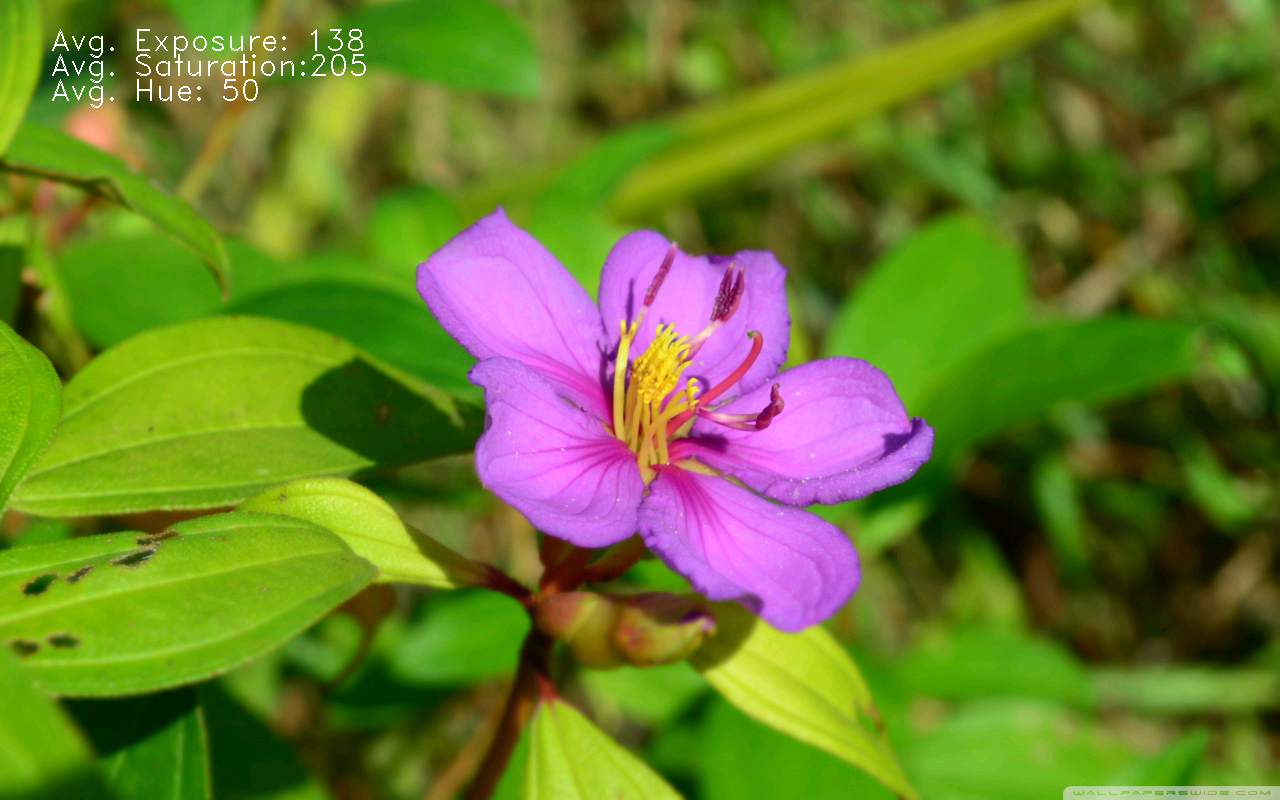
\includegraphics[scale=0.25]{experiment1.png}
	\caption{Experiment displaying average values of hue, saturation and value calculated with equation \ref{eq:average_hsv}\cite{Datta}.}
	\label{fig:experiment1}
\end{figure}

As a second experiment we experimented a visualization of detecting a triangular composition (Section \ref{subsub:rule_triangles}). In every frame received from the camera, the devices detects the first three faces and draws a triangle between them, serving as a visual cue for a better rearrangement of the subjects (Figure \ref{fig:experiment2}).

\begin{figure}[htbp]
    \centering
    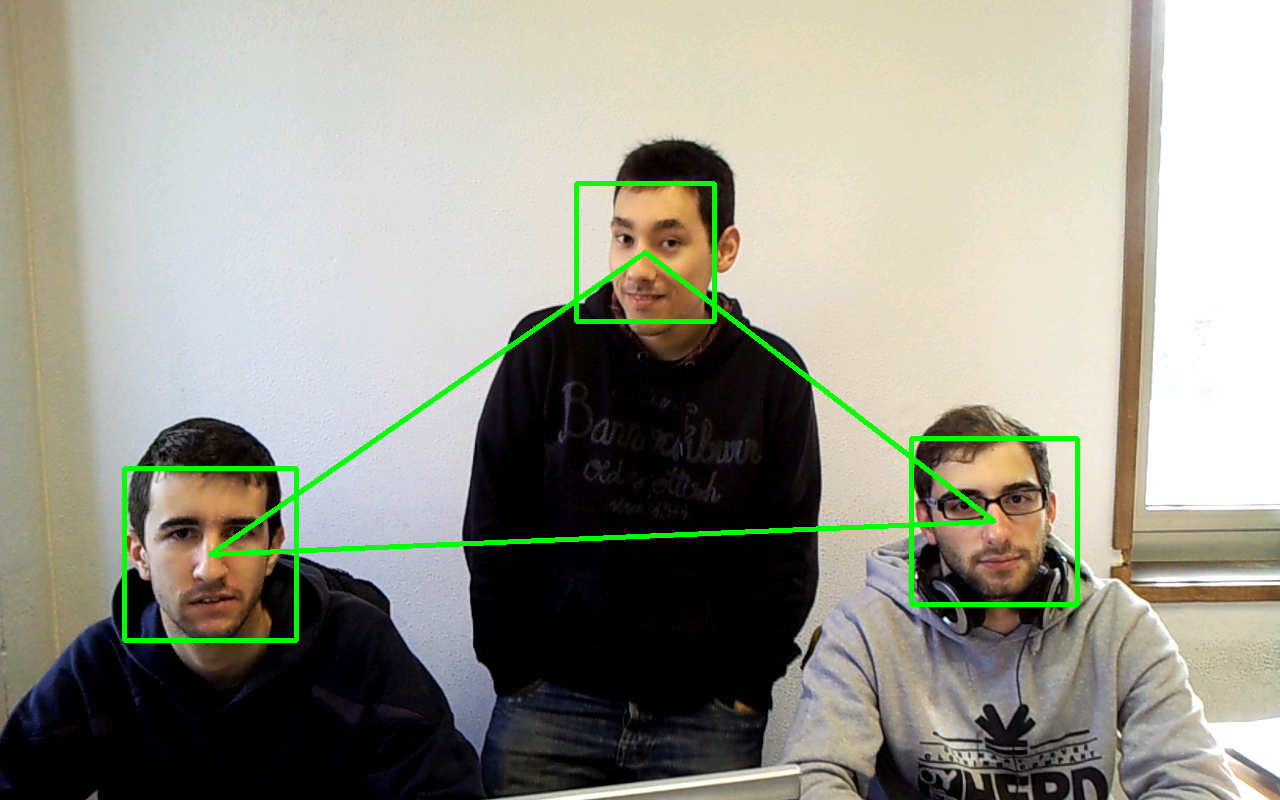
\includegraphics[scale=0.25]{experiment2.png}
	\caption{Experiment with triangle drawn with detected faces.}
	\label{fig:experiment2}
\end{figure}

This experiment was made using a Cascade Classifier in JAVA and C++ implemented by OpenCV. Both Cascade Classifiers used the same pre-trained classifier for frontal face detection. JAVA's classifier presented a better performance in both speed and detection. C++'s classifier was unable to detect faces between consecutive frames with minimum or without movement.
\subsection{Work Plan}